\clearpage{\pagestyle{empty}\cleardoublepage}

\chapter{Algoritmo di correzione dell'immagine}

\begin{flushright}\begin{small}\textit{"Any fool can write code that a computer can understand.\\
Good programmers write code that humans can understand."}\\
- Martin Fowler -\\
\end{small}\end{flushright}

Questo capitolo si propone di descrivere nei suoi tratti principali il software per l'elaborazione di immagini a fluorescenza sviluppato con tale progetto di tesi. 

L'algoritmo, scritto nel linguaggio di programmazione Python \cite{python}, ha lo scopo di ``ripulire'' le immagini acquisite col microscopio a fluorescenza da alcuni difetti di natura tecnico-sperimentale, connessi perlopiù alla sorgente di luce dello strumento (capitolo 2.2.3). 
In particolare le correzioni apportate all'immagine sono mirate all'eliminazione dell'``effetto dei bordi'' e della fluorescenza di background. 
Infatti, come si evince dalla \figurename~\ref{fig:bordi}, ogni immagine a fluorescenza è inevitabilmente affetta da una luminosità residua di sfondo, causata dalla necessità di una sorgente di luce per l'eccitazione del campione, e da una luminescenza disomogenea, intrinsecamente connessa all'irregolarità spaziale dell'illuminazione della sorgente.
Quest'ultimo difetto è quello che grava maggiormente su un'eventuale analisi quantitativa dell'immagine e, poiché ineliminabile dal punto di vista pratico-operazionale, è possibile affrontarlo unicamente tramite un'elaborazione via software. 

\begin{figure}
 \centering
 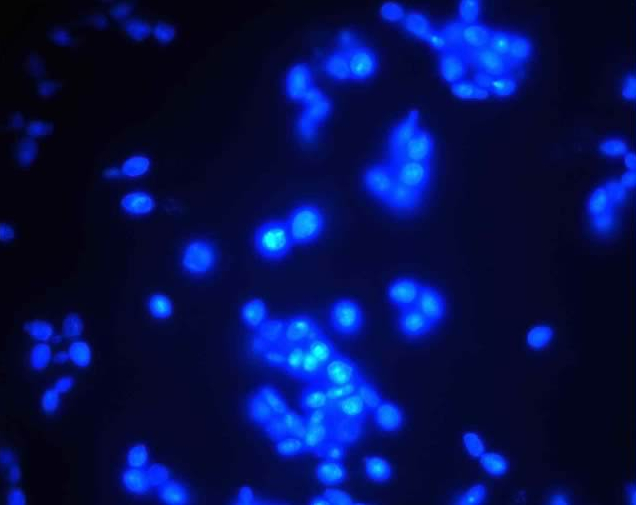
\includegraphics[scale=.40]{img/CAP3bordi.jpg}
 \caption{\small{Immagine in colorazione DAPI di cellule di lievito osservate al microscopio a fluorescenza.}}
 \label{fig:bordi}
\end{figure}

Per poter usufruire di tale programma è necessario disporre di un set di microsfere standards di riferimento in grado di generare una serie ben definita di livelli di intensità, così da poter creare curve di calibrazione e valutare la luminosità del campione. 
Nel nostro caso si è sfruttato il kit di microsfere fluorescenti nel rosso ``InSpeck Microscope Image Intensity Calibration'', messo a disposizione dal Dipartimento di Fisica di Bologna. 
Esso consiste in una fiala di $5\ ml$ di mezzo di coltura e 7 fiale di microsfere di polistirene: in una non fluorescenti e nelle altre con intensità relativa di fluorescenza lungo una scala pressochè logaritmica, ossia pari a 0.3\%, 1\%, 3\%, 10\%, 30\%, 100\%.
Tale richiesta nasce dal fatto che l'algoritmo effettua la correzione dell'immagine a fluorescenza delle cellule sfruttando l'ulteriore acquisizione di due immagini di calibrazione: una di sferette con stessa intensità e l'altra di sferette con 5 intensità differenti.

Descriviamo dunque passo a passo le fasi principali dell'algoritmo, riportato nella sua interezza in Appendice A.

\section{Rimozione dell'``effetto dei bordi''}

Come precedentemente osservato, l'``effetto dei bordi'' consiste nell'ottenimento di immagini a microscopia a fluorescenza con maggior luminosità della zona centrale rispetto a quella di confine. 
L'algoritmo mira alla rimozione di tale difetto richiedendo l'inserimento da parte dell'utente di una prima immagine di calibrazione, ossia quella delle sferette con un'unica intensità (\figurename~\ref{fig:unaint}).

\begin{figure}
 \centering
 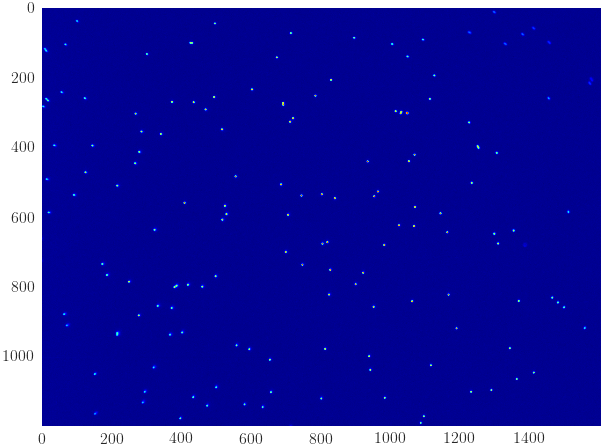
\includegraphics[scale=1]{img/CAP3unaint.png}
 \caption{\small{Immagine 1600x1200 pixel a fluorescenza di sferette con intensità relativa del 10\%.}}
 \label{fig:unaint}
\end{figure}

Inizialmente il programma applica su di essa il filtro gaussiano, tipico filtro di smoothing molto efficace per attenuare il rumore presente, e calcola in un primo modo approssimato l'intensità costante residua.
Questo background viene valutato in modo statistico come massimo delle mode, ossia dei valori che compaiono più frequentemente, di ogni riga della matrice bidimensionale che costituisce l'immagine. 
Una volta calcolato, tale parametro viene sottratto a quest'ultima poiché valore costante in grado di alterare considerazioni quantitative.

Successivamente si cercano le coordinate dei massimi dell'immagine, identificati dai centri delle varie sferette, tramite la funzione \textit{find\_max}. 
Essa applica filtri di massimo e minimo basandosi sulle variabili \textit{vicinanza\_size} e \textit{soglia}, il cui valore dovrà essere opportunatamente variato a seconda del campione di riferimento. 
La prima dà la dimensione in pixel dell'area sfruttata dai filtri per la ricerca dei massimi e dei minimi relativi, perciò dovrà assumere valori minori al crescere della concentrazione delle sferette. 
La seconda invece entra in gioco nella determinazione vera e propria dei centri delle sferette, infatti un pixel viene riconosciuto come punto di massimo solamente se, dopo la sottrazione dei due filtri, il suo valore risulta maggiore rispetto a quello della variabile. 
Di conseguenza tale parametro dipende dalla luminosità di sfondo: maggiore sarà il background e maggiore dovrà essere il suo valore.
Inoltre va sottolineato il fatto che dalla ricerca dei massimi viene escluso il confine dell'immagine, utilizzando il parametro \textit{margine}. 
Tale scelta è stata fatta perché ogni sferetta non viene rappresentata come punto oggetto, bensì con un cerchio di confusione (capitolo 2.2.1) e di conseguenza, nel caso in cui l'alone sia a cavallo del margine dell'immagine, potrebbe venire riconosciuto come massimo un punto che in realtà non è il centro della sferetta ma un pixel della sfumatura circostante.
Sempre all'interno di \textit{find\_max} viene associata ad ogni punto di massimo un'intensità integrale media. 
Questa viene calcolata richiamando la funzione \textit{intensity}, la quale somma i valori dei pixel che costituiscono la sferetta e divide il tutto per il numero totale di pixel contati, così da tener conto del fatto che non si tratta di un punto oggetto privo di dimensioni, bensì di un'area con una certa estensione. 
Per fare ciò ovviamente è necessario stimare il raggio \textit{delta} della sferetta, nel nostro caso corrispondente a 5 pixel.

\begin{figure}
 \centering
 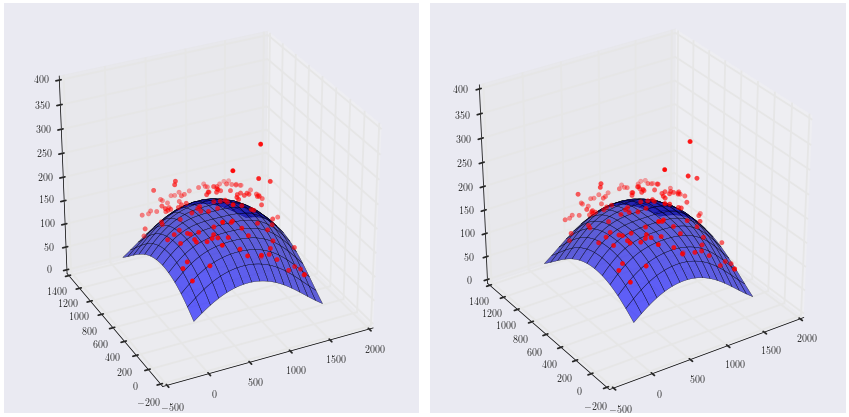
\includegraphics[scale=0.50]{img/CAP3gauss.png}
 \caption{\small{In rosso sono rappresentati i massimi della \figurename~\ref{fig:unaint} ed in nero è raffigurata la superficie risultante dal fit.}}
 \label{fig:gauss}
\end{figure}

Il passo successivo sta nell'utilizzo della funzione \textit{analyze} per il fit dei punti di massimo. 
Dopo varie analisi si è notato che la funzione che al meglio descrive il comportamento dei massimi di intensità è una funzione di tipo esponenziale, simile ad una gaussiana, descritta dal valore di return della funzione \textit{gauss}. 
Essendo questa uno dei punti cardine della correzione, si è deciso di parallelizzarla, così da avere un guadagno nei tempi e nell'affaticamento dei core di almeno quattro volte.
Una volta ottenuti i parametri della funzione ciò che si viene a creare è una superficie tridimensionale con forma analoga a quella riportata in \figurename~\ref{fig:gauss}. 
Quest'ultima immagine mette bene in evidenza il fatto che alcuni punti di massimo corrispondono ad intensità molto elevate rispetto alla media, pur trattandosi di sferette con medesima intensità relativa.
Questo fenomeno è da associarsi alla possibilità che due sferette possano trovarsi così vicine da apparire sovrapposte ed essendo questa un'alterazione dei risultati è necessario rieseguire il calcolo dei parametri dopo aver eliminato tali punti più intensi. 
Per fare ciò viene utilizzato il quantile$_{0.95}$, ossia vengono eliminati dal nuovo fit quei pixel con intensità superiore ad esso, pari per definizione al 5\% dei massimi inizialmente rilevati.
I nuovi parametri ottenuti a questa seconda iterazione sono restituiti dalla funzione \textit{analyze} e risultano essere la chiave per la correzione dell'effetto dei bordi di una qualunque immagine a fluorescenza, anche la stessa di calibrazione (\figurename~\ref{fig:unaintcorr}).
Infatti a questo punto inserendo una qualsiasi immagine come variabile di ingresso della funzione \textit{correction} è possibile eliminare tale difetto sulla base dei soli parametri del fit precedentemente calcolati. 
Tale funzione è molto semplice poiché sfrutta la normalizzazione del valore dei pixel dell'immagine sulla base del valore previsto dalla superficie tridimensionale.

\begin{figure}
 \centering
 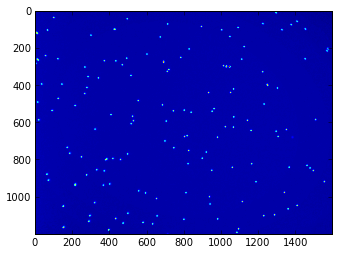
\includegraphics[scale=1]{img/CAP3unaintcorr.png}
 \caption{\small{Immagine corretta dall'``effetto dei bordi'' della \figurename~\ref{fig:unaint}.}}
 \label{fig:unaint}
\end{figure}

Tramite questa prima fase, che sfrutta la sola immagine di calibrazione di sferette con stessa intensità, si riesce quindi a eliminare in modo sostanziale ogni tipo di dipendenza dell'intensità dalla posizione del pixel. 

\section{Rimozione della fluorescenza di background}



\section{Correzione dell'immagine}


